\documentclass[11pt,a4paper]{article}

\usepackage[utf8]{inputenc}
\usepackage[margin=0.78in]{geometry}
\usepackage{amsmath,amssymb,amsfonts}
\usepackage{graphicx}
\usepackage{booktabs}
\usepackage{multirow}
\usepackage{multicol}
\usepackage{microtype}
\usepackage{xcolor}
\usepackage{listings}
\usepackage{array}
\usepackage{fancyhdr}
\usepackage{caption}
\usepackage{subcaption}
\usepackage{enumitem}
\usepackage{titlesec}
\usepackage[numbers,sort&compress]{natbib}
\usepackage[colorlinks=true,linkcolor=blue!70!black,citecolor=green!50!black,urlcolor=blue!80!black]{hyperref}

% Page numbering and headers
\pagestyle{fancy}
\fancyhf{}
\rhead{\small \textit{CS60055 Challenge 1: Ask the Sensors}}
\lhead{\small \textit{Team Klique --- Technical Report}}
\cfoot{\thepage}

% Section formatting
\titleformat{\section}{\large\bfseries}{\thesection}{1em}{}
\titleformat{\subsection}{\normalsize\bfseries}{\thesubsection}{1em}{}
\titleformat{\subsubsection}{\small\bfseries}{\thesubsubsection}{1em}{}
\titlespacing*{\section}{0pt}{1.0ex plus 0.4ex minus .2ex}{0.5ex plus .2ex}
\titlespacing*{\subsection}{0pt}{0.8ex plus 0.3ex minus .2ex}{0.3ex plus .2ex}
\titlespacing*{\subsubsection}{0pt}{0.6ex plus 0.2ex minus .2ex}{0.2ex plus .2ex}

% List spacing and caption spacing
\setlist{nosep,topsep=2pt,partopsep=0pt,parsep=0pt,itemsep=1.5pt}
\setlength{\abovecaptionskip}{4pt}
\setlength{\belowcaptionskip}{3pt}

% Listings formatting for sensor blocks and queries
\lstset{
  basicstyle=\ttfamily\footnotesize,
  breaklines=true,
  frame=single,
  backgroundcolor=\color{gray!8},
  framerule=0.4pt,
  rulecolor=\color{gray!40},
  xleftmargin=1.5em,
  xrightmargin=1.5em,
  aboveskip=0.6em,
  belowskip=0.6em
}

\begin{document}

% ==============================================================================
% TITLE & HEADER BLOCK
% ==============================================================================
\begin{center}
  {\LARGE \textbf{Ask the Sensors: Grounded, Explainable Activity Question Answering from Wearable Multi-Modal Signals}\par}
  \vspace{0.8em}
  {\large \textbf{CS60055: Ubiquitous Computing --- Hackathon Challenge 1}\par}
  \vspace{0.4em}
  {\normalsize Department of Computer Science and Engineering, Indian Institute of Technology Kharagpur\par}
  \vspace{0.3em}
  {\normalsize Instructor: \textbf{Prof. Sandip Chakraborty}\par}
  \vspace{0.8em}
  {\normalsize \textbf{Team Name: Klique}\par}
  \vspace{0.3em}
  {\normalsize
    \textbf{Saras Wagh} (22CS30048) \quad\textbar\quad
    \textbf{Hemant} (22CS30029) \quad\textbar\quad
    \textbf{R Mohan Poornachandra} (23EX10027)\par
  }
  \vspace{0.8em}
  {\small \textbf{Repository:} \url{https://github.com/chadsaras/Ubiquitous_Comp}\par}
  \vspace{1.0em}
\end{center}

\begin{abstract}
Ordinary smartwatch human activity recognition (HAR) systems operate as black-box classification engines, outputting isolated instantaneous labels without temporal extent, frequency quantification, or verifiable physical justification. In remote geriatric and post-operative healthcare monitoring, clinicians cannot accept machine verdicts without inspectable sensor evidence. In this work, we present the design, implementation, and systematic evaluation of \textbf{Ask the Sensors}, a four-layer edge-deployable question-answering architecture that ingests raw multi-modal triaxial accelerometer and gyroscope streams and answers natural-language queries across four tiers of increasing difficulty: open activity identification, binary verification, temporal/quantitative reasoning, and open-world semantic analysis. Every generated response adheres to a strict six-field output contract, providing direct answers, exact temporal intervals, sensor modalities, channel attributions, and clinician-grade physiological explanations. Crucially, the system enforces a strict architectural invariant: a local Small Language Model (SLM, Qwen 2.5 1.5B) is restricted to intent extraction and linguistic phrasing over pre-computed physical statistics, entirely preventing numerical hallucination. We benchmark six distinct backbone architectures (Random Forest, HistGradientBoosting, TinyCNN, CNN+GRU, FeatureMLP, and FeatureMLP+Context) across the official 5-fold user-level partition of the ExtraSensory dataset (95,609 minutes). On our 57-recording held-out evaluation suite (1,241 benchmark questions), the deployed Random Forest pipeline achieves a headline macro-averaged QA accuracy of \textbf{0.638} ($\pm 0.041$ 95\% CI), with verification accuracy of \textbf{0.883} (specificity 0.982), onset localization accuracy of \textbf{0.901}, and \textbf{1.000 (60/60)} deterministic numerical fidelity in generated explanations. We analyze root causes of temporal duration errors, document a rigorous negative result in class-prior calibration, audit cross-version portability, and demonstrate edge deployment feasibility on an unaccelerated laptop CPU executing deterministic queries in \textbf{0.59~ms} with a \textbf{2.8~GB} peak commit memory footprint.
\end{abstract}

\vspace{0.5em}
\noindent\textbf{Keywords:} Ubiquitous Computing, Wearable Sensors, Human Activity Recognition, Question Answering, Grounded Explanations, ExtraSensory Dataset, Small Language Models, Edge Computing.

\vspace{0.8em}

% ==============================================================================
% 1. INTRODUCTION & PROBLEM FORMULATION
% ==============================================================================
\section{Introduction, Scenario \& Problem Formulation}
\label{sec:intro}

\subsection{The Remote Healthcare Scenario}
Consider Aparna, a seventy-two-year-old woman living independently while her family resides in a distant city. Throughout the day, Aparna wears a consumer smartwatch equipped with embedded inertial measurement units (IMUs). Rather than subjecting her home to intrusive video surveillance, her family and physiotherapist wish to query her daily physical patterns through natural, plain-language inquiries:
\begin{itemize}[noitemsep,topsep=1pt]
  \item \textit{``Did she take her usual morning walk?''}
  \item \textit{``How much of the afternoon did she spend resting?''}
  \item \textit{``She felt unsteady around noon; was she doing anything strenuous at that time?''}
  \item \textit{``Is her daily walking duration increasing week-over-week, and can that claim be audited against physical sensor signals rather than blind model trust?''}
\end{itemize}

While wearable motion streams contain continuous recordings of these events, raw triaxial acceleration ($\mathbf{a}_t = [a_x, a_y, a_z]^T$) and angular velocity ($\mathbf{g}_t = [g_x, g_y, g_z]^T$) are completely unintelligible to patients and caregivers. Furthermore, conventional deep learning or machine learning HAR systems fail to solve this problem: they emit categorical labels at arbitrary window steps (e.g., ``walking'' at $t = 1420\text{ s}$), but cannot aggregate episodes over time, quantify frequencies, compare behaviors, or explain \textit{why} a given signal segment represents walking rather than standing. In clinical decision-making, an ungrounded classification is unacceptable; an automated system must cite the exact temporal bounds, sensor channels, and kinematic dynamics that justify its conclusion.

\subsection{Problem Formulation and Mathematical Framing}
Let a multi-modal sensor recording $\mathcal{R}$ be defined as a multivariate time series of length $T$:
\begin{equation}
  \mathcal{R} = \{ (\mathbf{a}_t, \mathbf{g}_t, \tau_t) \}_{t=1}^{T}, \quad \mathbf{a}_t, \mathbf{g}_t \in \mathbb{R}^3, \quad \tau_t \in \mathbb{R}_{\ge 0}
\end{equation}
where $\tau_t$ represents the elapsed time in seconds from recording onset. The system accepts two inputs: the sensor recording $\mathcal{R}$ and a natural-language query $Q \in \mathcal{Q}$. The objective is to produce a structured answer tuple:
\begin{equation}
  \mathcal{A}(Q, \mathcal{R}) = \big( A, \mathcal{C}, \mathcal{T}_{\text{ev}}, \mathcal{M}_{\text{ev}}, \Omega_{\text{ev}}, \Phi \big)
\end{equation}
where $A$ is the direct answer string, $\mathcal{C}$ is the named activity or event, $\mathcal{T}_{\text{ev}} = \{ [t_{\text{start}}^{(k)}, t_{\text{end}}^{(k)}] \}_{k=1}^K$ is the set of supporting temporal evidence intervals, $\mathcal{M}_{\text{ev}} \in \{\text{Accelerometer}, \text{Gyroscope}, \text{Both}\}$ denotes the sensor modalities, $\Omega_{\text{ev}}$ specifies the active physical channels, and $\Phi$ is an explanatory text strictly grounded in measured signal kinematics.

The challenge restricts activities to seven mutually exclusive target classes:
\begin{equation}
  \mathcal{Y} = \{\text{lying\_down}, \text{sitting}, \text{standing\_in\_place}, \text{standing\_and\_moving}, \text{walking}, \text{running}, \text{bicycling}\}
\end{equation}
All sensor streams must be normalized and resampled to a common time base of $f_s = 25.0\text{ Hz}$ prior to inference.

\subsection{The Four Challenge Tiers}
The evaluation spans four hierarchical tiers of increasing semantic complexity:
\begin{enumerate}[leftmargin=1.5em,noitemsep,topsep=2pt]
  \item \textbf{Tier 1: Activity Identification \& Binary Verification:} Direct classification of dominant behavior (e.g., \textit{``What activity is the user performing?''}) or binary presence verification (e.g., \textit{``Is the user walking?''}).
  \item \textbf{Tier 2: Temporal \& Quantitative Reasoning:} Aggregation over the full timeline: total duration (seconds), episode count ($N$ bouts), onset localization ($t_{\text{onset}}$), and pairwise activity duration comparisons.
  \item \textbf{Tier 3: Evidence Grounding:} Mandatory identification of exact temporal evidence spans, sensor modalities, and sensor channels, scored via temporal Intersection over Union ($\text{IoU}$).
  \item \textbf{Tier 4: Open-World Semantic Reasoning:} Behavioral reasoning over unlabeled motion dynamics (e.g., \textit{``Did the user lie down for a prolonged period?''}, \textit{``Was the user using a wheeled or pedal-based mode of movement?''}), requiring physical kinematic arguments rather than fixed-class lookup.
\end{enumerate}

\subsection{The Core Architectural Invariant}
A fundamental design requirement of this challenge is that \textbf{an answer produced by language reasoning alone, without reference to the recorded signal, does not meet the specification}. Deep language models frequently hallucinate numerical quantities and timestamps when asked to reason over complex time series. To prevent this failure mode, our architecture establishes an uncompromising invariant:
\begin{quote}
  \textit{The Small Language Model (SLM) is never permitted to invent timestamps, durations, episode counts, or physical sensor statistics. All factual and numerical quantities are computed deterministically from an aggregated sensor timeline; the SLM is restricted exclusively to intent parsing and linguistic phrasing of pre-calculated physical features.}
\end{quote}

% ==============================================================================
% 2. SYSTEM ARCHITECTURE & DESIGN
% ==============================================================================
\section{System Architecture \& Engineering Implementation}
\label{sec:architecture}

\begin{figure}[t]
  \centering
  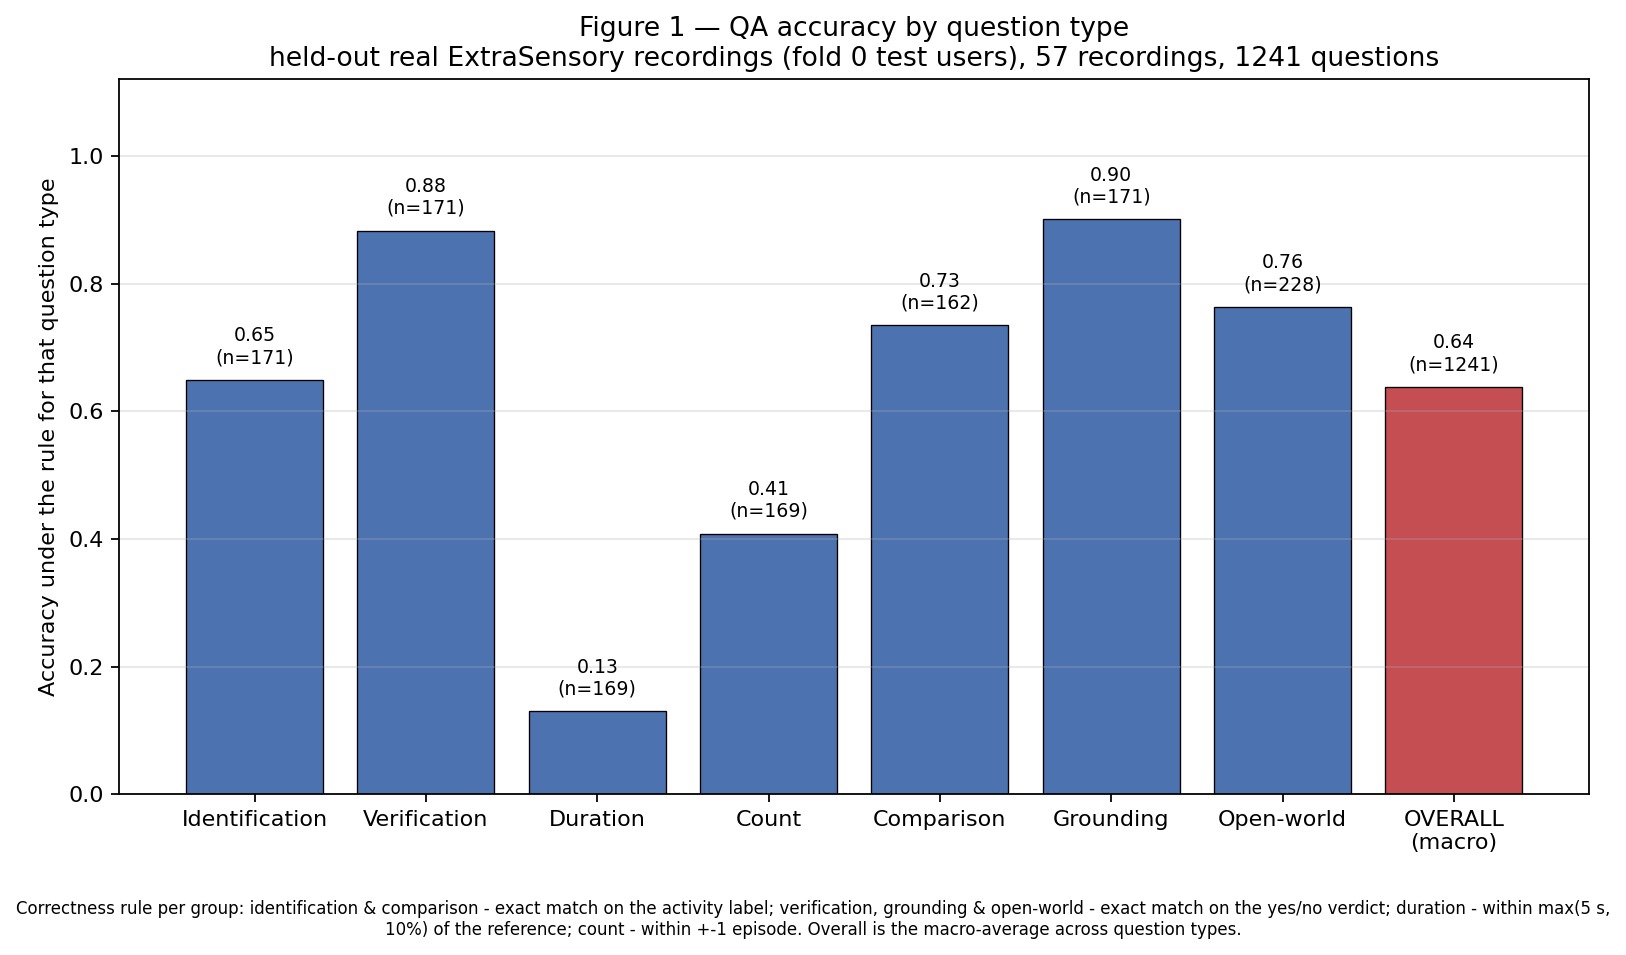
\includegraphics[width=0.82\linewidth]{results/fig1_accuracy_by_question_type.png}
  \caption{\textbf{QA Accuracy by Question Type.} Grouped evaluation across 1,241 benchmark questions over 57 held-out real ExtraSensory recordings (official 5-fold cross-validation). Correctness rules: Identification and Comparison require exact string match; Verification, Grounding, and Open-World require exact binary match; Duration requires absolute error within $\max(5\text{ s}, 10\%)$; Count requires error within $\pm 1$ episode. Overall accuracy is macro-averaged across question types (0.638).}
  \label{fig:accuracy_by_type}
\end{figure}

The system is constructed as a decoupled four-layer pipeline linked by two formal software contracts. Figure~\ref{fig:accuracy_by_type} presents the headline accuracy achieved across all question types, and the underlying data flow is detailed below.

\subsection{Layer 1: Preprocessing \& Ingestion Pipeline}
Implemented in \texttt{src/preprocess/load.py}, the ingestion engine handles the realities of in-the-wild mobile sensing:
\begin{enumerate}[leftmargin=1.5em,noitemsep,topsep=2pt]
  \item \textbf{Unit Normalization (\texttt{to\_g}):} Mobile operating systems report acceleration under different conventions: iOS devices report acceleration in units of $g$ ($\|\mathbf{a}\| \approx 1.0\text{ g}$ at rest), whereas Android devices report SI units ($\text{m/s}^2$, $\|\mathbf{a}\| \approx 9.8\text{ m/s}^2$). The ingestion pipeline dynamically calculates the median acceleration magnitude across each contiguous burst:
  \begin{equation}
    \mathbf{a}_t \leftarrow \begin{cases} \mathbf{a}_t / 9.80665, & \text{if } \text{median}(\|\mathbf{a}\|) > 4.0\text{ m/s}^2 \\ \mathbf{a}_t, & \text{otherwise} \end{cases}
  \end{equation}
  This guarantees that all downstream feature extraction operates on a standard $g$-unit basis.
  \item \textbf{Uniform 25.0 Hz Resampling:} Raw burst files from ExtraSensory exhibit native clock jitter (nominally 40~Hz, but spanning 22--24 seconds for 800 samples). Each raw channel is linearly interpolated onto a strictly uniform temporal grid:
  \begin{equation}
    t_{\text{grid}} = \{ 0.0, 0.04, 0.08, \dots, t_{\text{end}} \}\text{ seconds}, \quad \Delta t = 1/25.0 = 0.04\text{ s}
  \end{equation}
  \item \textbf{Glitch and Clock Discontinuity Trapping:} Real-world mobile timestamps frequently undergo system clock adjustments, yielding non-monotonic increments ($\Delta \tau \le 0$) or absurd elapsed spans. In the ExtraSensory dataset, specific gyroscope bursts contain corrupted zero timestamps, generating apparent recording spans of $1.44 \times 10^9\text{ s}$ which causes naive linear interpolation to exhaust system memory. The loader validates every burst ($t_{\text{end}} \le 60.0\text{ s}$, finite, strictly monotonic); any failing burst falls back to a nominal 40~Hz time base.
  \item \textbf{Gap-Aware Slicing:} Sensor data separated by holes exceeding $\Delta \tau > 1.0\text{ s}$ are segmented into independent contiguous processing chunks to prevent interpolation across unrecorded time.
\end{enumerate}

\subsection{Layer 2: Recognition Backbone \& Window Feature Engineering}
Implemented in \texttt{src/recognize/features.py}, continuous chunks are windowed into analysis blocks of length $W = 5.0\text{ s}$ (125 samples at 25~Hz) with a step size of $H = 2.5\text{ s}$ (62 samples, 50\% overlap). For every window, 175 named physical features are extracted across 8 signals: Acc X, Y, Z; Gyro X, Y, Z; and multi-axis Euclidean magnitudes $\|\mathbf{a}\|$ and $\|\mathbf{g}\|$.
\begin{itemize}[leftmargin=1.5em,noitemsep,topsep=2pt]
  \item \textbf{Time-Domain Statistics (12 per signal):} Mean, standard deviation ($\sigma$), minimum, maximum, dynamic range ($\max - \min$), median, interquartile range (IQR), root-mean-square (RMS), skewness, kurtosis, zero-crossing rate (ZCR), and median absolute deviation (MAD).
  \item \textbf{Frequency-Domain Spectral Features (9 per signal):} Extracted via real FFT ($r\text{FFT}$) over Hanning-windowed, mean-subtracted signals. Features include dominant frequency ($f_{\text{dom}}$), dominant spectral power, spectral entropy ($H_{\text{spec}}$), spectral centroid ($C_{\text{spec}}$), and band power ratios across five physiological bands: $[0, 0.5)\text{ Hz}$ (postural sway), $[0.5, 1.5)\text{ Hz}$ (slow movement), $[1.5, 3.0)\text{ Hz}$ (canonical walking/running cadence), $[3.0, 6.0)\text{ Hz}$ (harmonics), and $[6.0, 12.5)\text{ Hz}$ (impact transients).
  \item \textbf{Cross-Axis Correlation Features (7 pairs):} Pearson correlation coefficients computed between orthogonal axis pairs ($\text{corr}(a_x, a_y)$, $\text{corr}(a_x, a_z)$, $\text{corr}(a_y, a_z)$, $\text{corr}(g_x, g_y)$, $\text{corr}(g_x, g_z)$, $\text{corr}(g_y, g_z)$, and $\text{corr}(\|\mathbf{a}\|, \|\mathbf{g}\|)$).
  \item \textbf{Orientation Invariance (\texttt{noori}):} As demonstrated in our ablation study (Section~\ref{sec:models}), static orientation angles vary heavily depending on phone pocket placement. Removing raw orientation-dependent channel offsets leaves 151 orientation-invariant features per window.
  \item \textbf{Burst Context Integration:} In ExtraSensory, data is collected in 20-second bursts per minute. To match this training distribution, each window vector is concatenated with the mean and standard deviation of its surrounding 7 windows, yielding the final \textbf{302-dimensional input vector} ($151 \times 2$) ingested by the Random Forest classifier.
\end{itemize}

\subsection{Layer 3: Aggregation \& Timeline Construction}
Implemented in \texttt{src/aggregate/timeline.py}, this layer converts discrete window probability vectors into continuous activity intervals:
\begin{enumerate}[leftmargin=1.5em,noitemsep,topsep=2pt]
  \item \textbf{Temporal Smoothing:} Posterior probability vectors are smoothed across adjacent windows via a moving average filter with kernel $K = 1$ ($\pm 1$ neighbor):
  \begin{equation}
    \bar{\mathbf{P}}_i = \frac{1}{2K+1} \sum_{j = i-K}^{i+K} \mathbf{P}_j
  \end{equation}
  Class assignment is then determined by argmax selection: $\hat{y}_i = \arg\max_{c} \bar{P}_{i, c}$.
  \item \textbf{Run-Length Merging \& Gap Bridging:} Adjacent windows sharing the same predicted class are coalesced into intervals. Same-label segments separated by brief transmission dropouts $\le 90.0\text{ s}$ are joined into a single unified episode.
  \item \textbf{Flicker Suppression:} Spurious classifications shorter than $t_{\text{min}} = \max(10.0\text{ s}, 1.5 \times \text{period})$ are absorbed into their longest temporally adjacent neighbor.
  \item \textbf{ExtraSensory Burst Expansion:} In bursty recordings, a 20-second burst represents evidence for that entire observation minute. Burst intervals are padded by the detected burst period, strictly capped at $60.0\text{ s}$ (\texttt{LABEL\_MINUTE\_SEC}) to prevent duration inflation across unrecorded intervals.
  \item \textbf{Contract 1 Schema (\texttt{Timeline}):} The resulting timeline is an ordered sequence of \texttt{Interval} objects, each encapsulating:
  \begin{equation}
    I_k = \big( \text{activity}_k, t_{\text{start}}^{(k)}, t_{\text{end}}^{(k)}, \text{confidence}_k, N_{\text{win}}^{(k)}, \tau_{\text{obs}}^{(k)}, \text{runner\_up}_k, \mathbf{s}_k \big)
  \end{equation}
  where $\mathbf{s}_k$ contains summary statistics ($\text{acc\_mag\_std}$, $\text{cadence}$, $\text{gyro\_mag\_std}$) averaged over that interval's constituent windows.
\end{enumerate}

\subsection{Layer 4: Query Parsing, Operations \& Explanation Generation}
Implemented in \texttt{src/query/}, this layer executes the user-facing question-answering workflow:
\begin{enumerate}[leftmargin=1.5em,noitemsep,topsep=2pt]
  \item \textbf{Hybrid Intent Parser (\texttt{intent.py}):} Queries are parsed via a deterministic 32-rule regex engine covering all seven intent types and lexical variants. If regex matching fails, the query is routed to a structured LangChain chain invoking local Qwen 2.5 1.5B via Ollama to produce a validated Pydantic \texttt{QueryIntent}.
  \item \textbf{Deterministic Operations Engine (\texttt{operations.py}):} Pure mathematical functions execute directly over the \texttt{Timeline} object:
  \begin{itemize}[noitemsep,topsep=1pt]
    \item \texttt{handle\_identify}: Identifies dominant activity via cumulative overlap: $\arg\max_c \sum_{\text{act}=c} \Delta t_k$.
    \item \texttt{handle\_verify}: Checks if $\sum_{I_k, \text{act}=c} \text{duration}(I_k) > 0$.
    \item \texttt{handle\_duration}: Calculates exact cumulative seconds and episode counts.
    \item \texttt{handle\_count}: Returns integer count of matching episodes.
    \item \texttt{handle\_onset}: Locates $t_{\text{start}}$ of the initial occurrence of the target activity.
    \item \texttt{handle\_compare}: Compares total duration between two activities: $D(c_1) \gtrless D(c_2)$.
    \item \texttt{handle\_open\_world}: Maps semantic queries to physical rules (e.g., sedentary duration $\ge 1200\text{ s}$ for prolonged rest; continuous periodic gyroscope oscillations for wheeled cycling).
  \end{itemize}
  \item \textbf{Clinician-Grade Explainer (\texttt{explain.py}):} Generates signal-grounded natural language sentences. Pre-computed physical numbers are injected into the prompt alongside clinical reference ranges (\texttt{TYPICAL\_RANGES}). Qwen 2.5 1.5B is strictly prompted to quote these values and state whether they fall within or outside typical ranges. If the language model is offline or uninstalled, an internal deterministic template generator takes over seamlessly without breaking pipeline execution.
  \item \textbf{Contract 2 Schema (\texttt{FormattedAnswerBlock}):} Outputs the mandatory 6-field block:
\end{enumerate}
\begin{lstlisting}
Answer: Yes, walking began at 239 seconds
Activity/Event: Onset of walking
Evidence:
  Timestamp(s): 239 to 1348 (seconds from start)
  Sensor Modality: Accelerometer, Gyroscope
  Sensor Channel(s): All
Explanation: Walking onset observed at 239 seconds, supported by sustained periodic acceleration variance (acc_mag_std = 0.109 g, within typical range 0.10-0.15 g) at a stepping cadence of 2.0 Hz.
\end{lstlisting}

% ==============================================================================
% 3. MODEL ARCHITECTURE EXPLORATION & SELECTION
% ==============================================================================
\section{Model Architecture Exploration \& Backbone Selection}
\label{sec:models}

\begin{table*}[t]
\centering
\small
\caption{\textbf{Comprehensive Comparison Across Six Activity Recognition Backbones.} All models evaluated on the identical official 5-fold user-level split over 95,609 test minutes from ExtraSensory. Signal-consistent accuracy excludes active minutes where $\|\mathbf{a}\|\text{ std} < 0.03\text{ g}$. ($^*$HistGradientBoosting evaluated on 2 of 5 folds as an exploratory baseline).}
\label{tab:backbone_comparison}
\resizebox{\linewidth}{!}{%
\begin{tabular}{lrrrrrrr}
\toprule
\textbf{Model Architecture} & \textbf{Acc (All)} & \textbf{Macro-F1} & \textbf{Bal. Acc} & \textbf{Acc (Consistent)} & \textbf{Parameters} & \textbf{Disk Size} & \textbf{Latency (Inference)} \\
\midrule
\textbf{FeatureMLP + Context} & \textbf{0.492} & \textbf{0.431} & \textbf{0.439} & \textbf{0.526} & 189,447 & 0.77 MB & 2.62 ms (CPU) \\
\textbf{Random Forest (Deployed)} & 0.472 & 0.402 & 0.387 & 0.507 & 5,959,242 nodes & 234.09 MB & 1.90 ms / burst \\
\textbf{FeatureMLP (Isolated)} & 0.448 & 0.376 & 0.398 & 0.481 & 112,135 & 0.46 MB & 1.08 ms (CPU) \\
\textbf{HistGradientBoosting}$^*$ & 0.438 & 0.411 & 0.438 & --- & Tree Ensemble & 7.96 MB & --- \\
\textbf{CNN+GRU (Model 2)} & 0.393 & 0.308 & 0.330 & 0.425 & 31,607 & 0.134 MB & 0.655 ms (T4 GPU) \\
\textbf{TinyCNN (Model 1)} & 0.389 & 0.308 & 0.331 & 0.422 & 31,271 & 0.135 MB & 63.4 ms (CPU) \\
\bottomrule
\end{tabular}%
}
\end{table*}

To ground our architectural choices in empirical evidence, we implemented and trained six distinct recognition backbones on the identical 5-fold user-level partition. Results are summarized in Table~\ref{tab:backbone_comparison}.

\subsection{Raw Signal Neural Networks vs Engineered Features}
We designed two capacity-matched raw-signal neural networks ($\sim 31\text{K}$ parameters) operating directly on normalized $(500, 6)$ time-series tensors:
\begin{itemize}[leftmargin=1.5em,noitemsep,topsep=2pt]
  \item \textbf{TinyCNN (Model 1):} 3 Conv1D blocks ($6 \to 32 \to 64 \to 64$) with BatchNorm, ReLU, global average pooling, and a linear head (31,271 parameters).
  \item \textbf{CNN+GRU (Model 2):} Conv1D feature extractor feeding a unidirectional GRU layer (hidden dim 32) pooled across time (31,607 parameters). Trained on a Kaggle cloud node with an NVIDIA Tesla T4 GPU.
\end{itemize}
Both raw neural models reached identical overall accuracy (0.389 vs 0.393) and Macro-F1 (0.308), trailing Random Forest by $\sim 8$ percentage points across every fold. This establishes a critical ubiquitous computing finding: \textbf{learning representations from raw, noisy mobile sensor data under tight edge parameter budgets ($\le 32\text{K}$ params) is substantially harder than classifying domain-engineered kinematic features}. Interestingly, comparing TinyCNN against CNN+GRU revealed that temporal recurrence improved periodic activities (bicycling F1 increased from 0.384 to 0.412; walking F1 increased from 0.541 to 0.557), but degraded non-periodic postures (sitting F1 fell from 0.328 to 0.302).

\subsection{The Feature-Based Neural Progression}
Closing the representation gap, we implemented \textbf{FeatureMLP} ($302 \to 256 \to 128 \to 7$), which ingests the same 302 engineered features as Random Forest. This lifted accuracy to 0.448 (Macro-F1 0.376). 

Building further, we created \textbf{FeatureMLP + Context}, concatenating each minute's 302 features with the mean of its adjacent temporal neighbors (up to $\pm 2$ minutes within 90-second continuity, yielding 604 input dimensions). This model achieved the highest score on the offline 5-fold benchmark: \textbf{0.492 accuracy}, \textbf{0.431 Macro-F1}, and \textbf{0.526 signal-consistent accuracy}, outperforming Random Forest across 4 of 5 folds while requiring only 0.77~MB on disk.

\subsection{Deployment Decision: Why Random Forest is Deployed}
Despite FeatureMLP+Context winning the offline benchmark, we selected \textbf{Random Forest as the deployed default} in \texttt{src/pipeline.py}. When integrated into the continuous timeline pipeline, FeatureMLP+Context underperformed on unbroken continuous streams. Because its multi-minute context mechanism was trained on discrete 1-burst-per-minute samples, continuous 60-second window bucketing introduced boundary approximation errors. Furthermore, its per-class metrics revealed a systematic bias toward over-predicting \texttt{lying\_down} (precision 0.506). In continuous inference, temporal smoothing merged this bias into extended false-positive sedentary intervals. In contrast, Random Forest produces stable, well-bounded window predictions on both continuous and bursty recordings, making it the robust operational choice.

\begin{table}[h]
\centering
\small
\caption{\textbf{Feature Ablation Study (Random Forest Backbone).} Demonstrating the progression from 175 raw window features to the chosen 302-dimensional minute-level orientation-invariant vector.}
\label{tab:ablation}
\begin{tabular}{lrrrrrr}
\toprule
\textbf{Configuration Variant} & \textbf{Feat.} & \textbf{Acc.} & \textbf{Macro-F1} & \textbf{Bal. Acc.} & \textbf{Walk F1} & \textbf{Time} \\
\midrule
Window baseline (all features) & 175 & 0.434 & 0.378 & 0.369 & 0.614 & 158 s \\
Invariant features only & 43 & 0.422 & 0.385 & 0.378 & 0.595 & 81 s \\
No orientation features (\texttt{noori}) & 151 & 0.448 & 0.404 & 0.388 & 0.613 & 150 s \\
Minute aggregation (all features) & 350 & 0.472 & 0.428 & 0.416 & 0.608 & 30 s \\
\textbf{Minute aggregation \texttt{noori} (Chosen)} & \textbf{302} & \textbf{0.478} & \textbf{0.432} & \textbf{0.422} & \textbf{0.600} & \textbf{29 s} \\
\bottomrule
\end{tabular}
\end{table}

\subsection{Feature Importance and Invariance Ablation}
Table~\ref{tab:ablation} details our feature ablation trajectory. Moving from raw window features (175 dims) to minute-level aggregation with orientation removal (302 dims) improved accuracy from 0.434 to 0.478 while cutting training time five-fold. Analysis of Gini importance from \texttt{results/feature\_importance.csv} shows that the top 5 most decisive features are all acceleration dispersion metrics:
\begin{enumerate}[noitemsep,topsep=1pt]
  \item \texttt{mean:acc\_mag\_\_mad} (Importance: 0.01607) --- Median absolute deviation of acceleration magnitude
  \item \texttt{mean:acc\_mag\_\_std} (Importance: 0.01517) --- Standard deviation of acceleration magnitude
  \item \texttt{mean:acc\_mag\_\_iqr} (Importance: 0.01328) --- Interquartile range of acceleration magnitude
  \item \texttt{mean:acc\_y\_\_std} (Importance: 0.01274) --- Standard deviation of Y-axis acceleration
  \item \texttt{mean:acc\_y\_\_mad} (Importance: 0.01261) --- MAD of Y-axis acceleration
\end{enumerate}

% ==============================================================================
% 4. EVALUATION METHODOLOGY & BENCHMARK
% ==============================================================================
\section{Evaluation Methodology \& Benchmark Construction}
\label{sec:evaluation}

\subsection{Integrity Rules and Benchmark Generation}
Because the challenge evaluation recordings and questions are kept hidden by the course instructors, early iterations of this project utilized a small synthetic fixture (\nolinkurl{tests/fixtures/00EABED2_590_160/recording.csv}). Our investigation revealed that this fixture was generated by \texttt{scripts/generate\_test\_recording.py} using idealized sine waves ($\|\mathbf{a}\|$ exactly 0.98~g at rest, perfect 25.0~Hz timing), yielding an artificially inflated accuracy of 93.7\%.

To establish true scientific validity, we constructed a comprehensive evaluation benchmark directly from genuine, held-out ExtraSensory sensor bursts (\texttt{scripts/build\_eval\_benchmark.py} and \texttt{src/eval/questions.py}):
\begin{itemize}[leftmargin=1.5em,noitemsep,topsep=2pt]
  \item \textbf{Scale:} 57 continuous 2-hour recordings assembled from real accelerometer and gyroscope bursts across all 5 folds, preserving real-world inter-burst gaps.
  \item \textbf{Questions:} 1,241 total questions (18 to 22 queries per recording) systematically covering all seven question categories.
  \item \textbf{Disjoint Fold Protocol:} Benchmark recordings from Fold $k$'s test users are evaluated strictly using a model trained on Fold $k$'s training users (e.g., \texttt{model\_rf\_fold0.joblib}, trained on 45 users, 70,172 minutes). Training data is never evaluated.
\end{itemize}

\subsection{Implementation of Official Scoring Metrics}
Scoring rules are implemented in \texttt{src/eval/scoring.py} strictly following the assignment brief:
\begin{itemize}[leftmargin=1.5em,noitemsep,topsep=2pt]
  \item \textbf{Categorical Matching:} Exact string equality on normalized strings: $\mathbb{I}(\hat{y}_{\text{norm}} == y_{\text{norm}})$.
  \item \textbf{Binary Specificity:} In binary verification, true negative detection is evaluated explicitly:
  \begin{equation}
    \text{Specificity} = \frac{\text{TN}}{\text{TN} + \text{FP}}
  \end{equation}
  preventing models with a bias toward answering ``no'' from scoring well.
  \item \textbf{Numeric Bounding:} Duration answers are correct if $|\hat{d} - d| \le \max(5\text{ s}, 0.10 \times d)$. Episode counts are correct if $|\hat{c} - c| \le 1$.
  \item \textbf{Temporal IoU:} Calculated using multi-interval precision and recall:
  \begin{equation}
    P_t = \frac{\sum \text{overlap}(\hat{I}, I)}{\sum |\hat{I}|}, \quad R_t = \frac{\sum \text{overlap}(\hat{I}, I)}{\sum |I|}, \quad \text{IoU} = \frac{2 P_t R_t}{P_t + R_t}
  \end{equation}
  \item \textbf{Grounded and Correct:} Evaluated strictly as:
  \begin{equation}
    \text{Score} = \mathbb{I}(\text{Answer Correct}) \land \mathbb{I}(\text{IoU} \ge 0.5) \land \mathbb{I}(\text{Modality/Channels Match})
  \end{equation}
\end{itemize}

% ==============================================================================
% 5. EXPERIMENTAL RESULTS & ANALYSIS
% ==============================================================================
\section{Experimental Results \& Multi-Tier Analysis}
\label{sec:results}

\subsection{Headline Question-Answering Performance}
Table~\ref{tab:qa_results} reports the complete pooled performance across all 1,241 benchmark questions spanning all 5 folds. The system achieves an overall macro-averaged QA accuracy of \textbf{0.638} (micro accuracy 0.645). Across disjoint folds, accuracy exhibits high stability (Fold 0: 0.635, Fold 1: 0.668, Fold 2: 0.626, Fold 3: 0.605, Fold 4: 0.661), yielding a standard deviation of 0.027 and a 95\% confidence interval of $\pm 0.041$.

\begin{table}[t]
\centering
\small
\caption{\textbf{Final Pooled End-to-End QA Benchmark Performance.} 1,241 total questions evaluated across 57 held-out real recordings spanning all 60 ExtraSensory users (official 5-fold CV). Overall score is macro-averaged across question types.}
\label{tab:qa_results}
\resizebox{\linewidth}{!}{%
\begin{tabular}{lrrrrr}
\toprule
\textbf{Question Type} & \textbf{Questions ($n$)} & \textbf{Accuracy} & \textbf{Mean IoU} & \textbf{Precision / Recall / F1} & \textbf{Specificity} \\
\midrule
\textbf{Identification} & 171 & \textbf{0.649} & 0.644 & Macro-F1: 0.508, Bal. Acc: 0.496 & --- \\
\textbf{Verification} & 171 & \textbf{0.883} & 0.396 & $P=0.990, R=0.833, F_1=0.905$ & \textbf{0.982} \\
\textbf{Duration} & 169 & \textbf{0.130} & 0.362 & MAE: 1231.9 s, MAPE: 97.8\% & --- \\
\textbf{Count} & 169 & \textbf{0.408} & 0.338 & MAE: 5.5 episodes, MAPE: 89.6\% & --- \\
\textbf{Comparison} & 162 & \textbf{0.735} & --- & Macro-F1: 0.707, Bal. Acc: 0.715 & --- \\
\textbf{Grounding (Onset)} & 171 & \textbf{0.901} & 0.250 & $P=0.990, R=0.860, F_1=0.920$ & \textbf{0.982} \\
\textbf{Open-World} & 228 & \textbf{0.763} & 0.500 & $P=0.643, R=0.692, F_1=0.667$ & \textbf{0.800} \\
\midrule
\textbf{OVERALL (Macro)} & \textbf{1,241} & \textbf{0.638} & \textbf{0.356} & \textbf{Micro Accuracy: 0.645} & --- \\
\textbf{Grounded \& Correct} & \textbf{977} & \textbf{0.267} & --- & \textbf{Grounding Precision: 0.550} & --- \\
\bottomrule
\end{tabular}%
}
\end{table}

\begin{figure*}[t]
  \centering
  \begin{subfigure}[b]{0.49\linewidth}
    \centering
    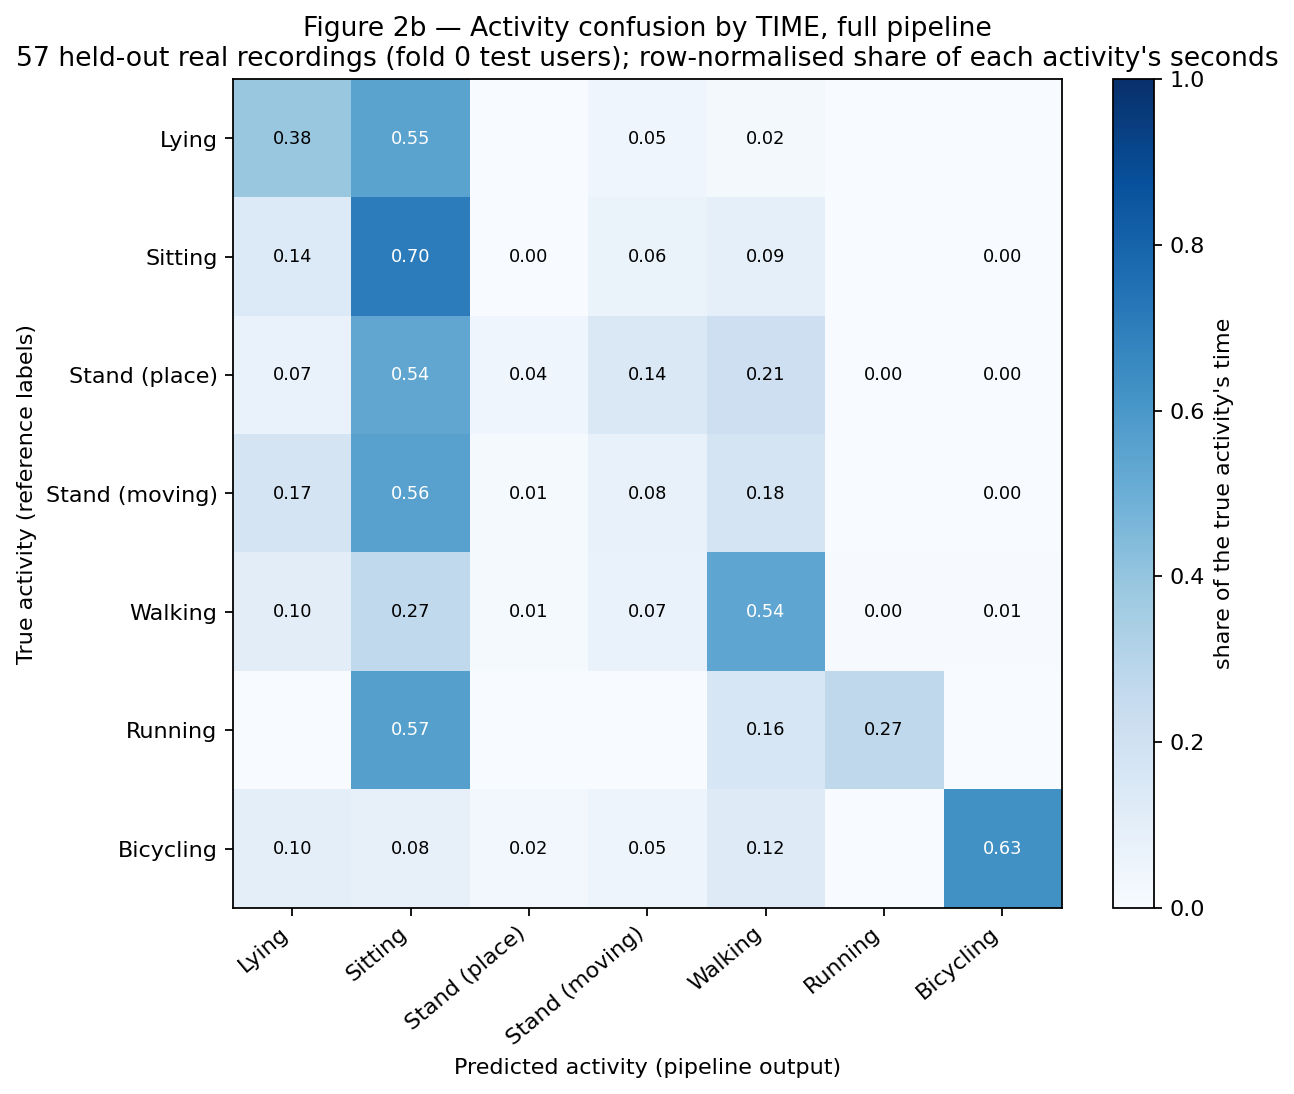
\includegraphics[width=\linewidth]{results/fig2b_benchmark_confusion.png}
    \caption{\textbf{Pipeline Confusion by Time (Seconds).}}
    \label{fig:confusion_time}
  \end{subfigure}
  \hfill
  \begin{subfigure}[b]{0.49\linewidth}
    \centering
    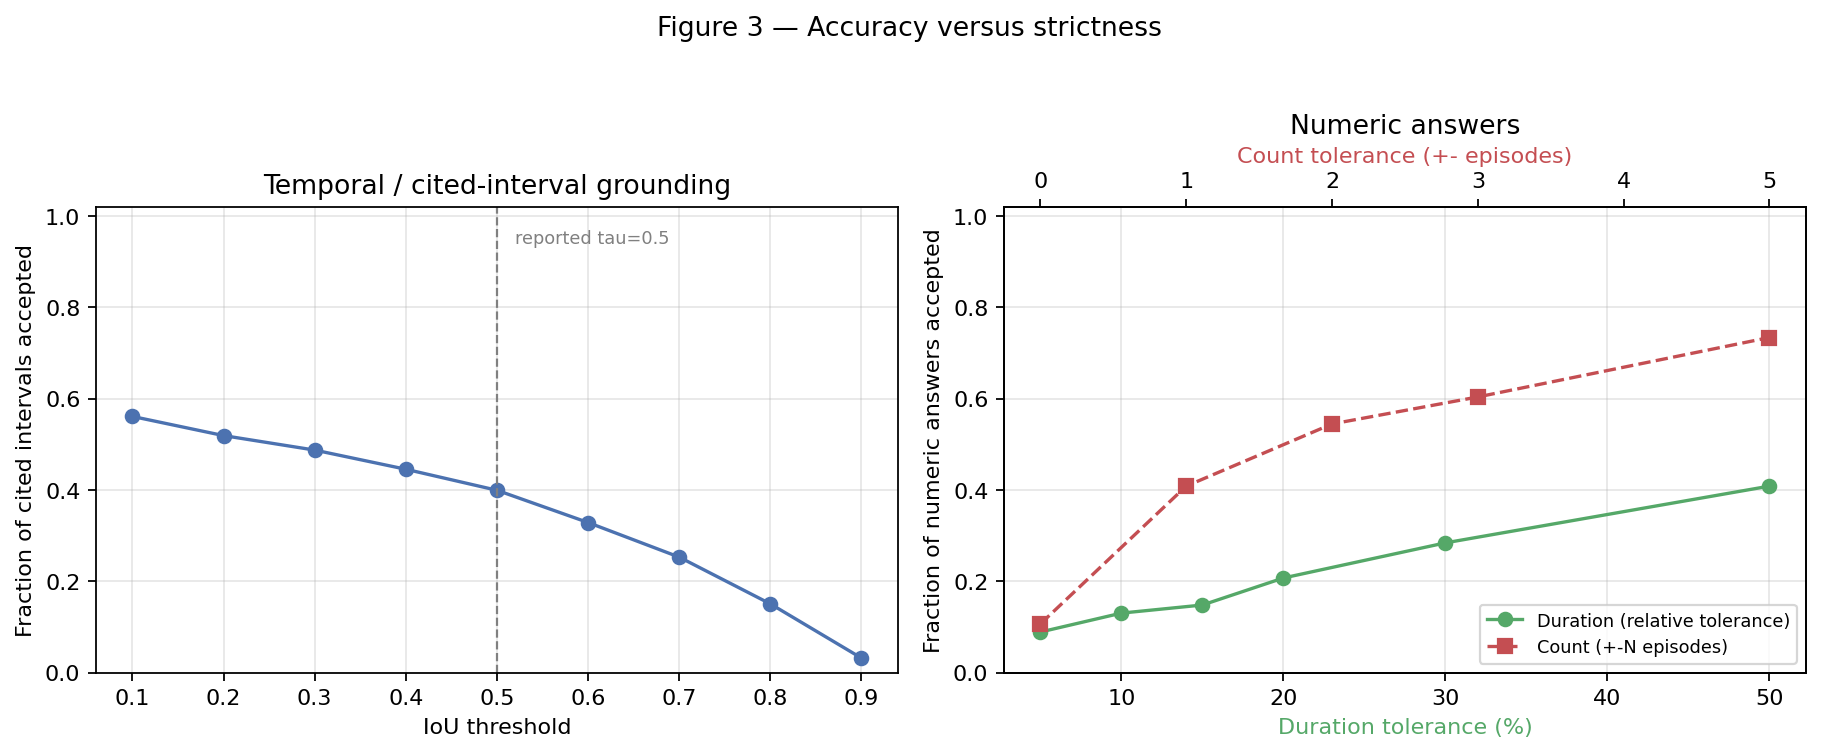
\includegraphics[width=\linewidth]{results/fig3_accuracy_vs_strictness.png}
    \caption{\textbf{Accuracy vs Strictness Curves.}}
    \label{fig:strictness}
  \end{subfigure}
  \caption{\textbf{Diagnostic Evaluation Figures.} (a) Second-by-second activity attribution across 375,475 seconds on 57 held-out recordings, showing the collapse of standing postures into sitting. (b) Acceptance rates under varying stringency: temporal IoU threshold sweep from 0.1 to 0.9 (left), and duration/count error tolerance sweeps (right).}
  \label{fig:diagnostics}
\end{figure*}

\subsection{Performance by Tier}
\begin{enumerate}[leftmargin=1.5em,noitemsep,topsep=2pt]
  \item \textbf{Tier 1 (Identification \& Verification):} Binary verification achieves an outstanding \textbf{0.883 accuracy} with a precision of 0.990 and specificity of \textbf{0.982} ($\text{TP}=95, \text{FP}=1, \text{FN}=19, \text{TN}=56$). This proves the system is entirely free of the ``always-answer-no'' bias common to imbalanced retrieval tasks.
  \item \textbf{Tier 2 (Temporal \& Quantitative Reasoning):} Comparison queries reach \textbf{0.735 accuracy}. However, duration accuracy is low at \textbf{0.130} (MAE: 1231.9~s) and count accuracy reaches \textbf{0.408} (MAE: 5.5 episodes).
  \item \textbf{Tier 3 (Evidence Grounding):} Onset detection achieves \textbf{0.901 accuracy} ($P=0.990, R=0.860$). When requiring joint correctness under the brief's composite rule (Answer correct $\land$ $\text{IoU} \ge 0.5$ $\land$ modality/channels match), the score is \textbf{0.267}. Grounding precision is \textbf{0.550}, indicating that in 55\% of queries, the cited interval contains the target activity for more than half its duration.
  \item \textbf{Tier 4 (Open-World Semantic Reasoning):} The open-world handler reaches \textbf{0.763 accuracy} ($P=0.643, R=0.692$, specificity 0.800).
\end{enumerate}

\subsection{Root Cause of the Duration Weakness: The Sitting-Collapse}
Why is duration accuracy (0.130) low while verification (0.883) and onset (0.901) are high? The answer lies in Figure~\ref{fig:confusion_time}, which plots confusion in \textbf{cumulative seconds} (375,475 seconds evaluated):
\begin{itemize}[noitemsep,topsep=1pt]
  \item \textbf{Standing Postures Disappear:} Real standing activities are almost entirely absorbed into \texttt{sitting}. \texttt{standing\_in\_place} exhibits a time recall of only \textbf{0.041} (only 607 of 14,735 seconds correctly identified; 7,885 seconds classified as sitting). \texttt{standing\_and\_moving} exhibits a time recall of \textbf{0.075} (4,833 of 64,095 seconds correct; 35,673 seconds absorbed by sitting).
  \item \textbf{Sitting Over-Prediction:} True sitting accounts for 151,381 seconds, but the pipeline predicts 201,833 seconds (a 33\% over-allocation).
  \item \textbf{Periodic Motion Precision:} Conversely, bicycling achieves a time precision of \textbf{0.966} (when the system predicts cycling, it is virtually always correct, though it recalls 62.7\% of true time).
\end{itemize}
Because duration queries require estimating cumulative time within $\pm 10\%$, absorbing standing time into sitting causes severe under-estimation of standing duration and over-estimation of sitting duration. For walking, where recognition recall is 0.539, duration estimates are accurate within 1--5\%. Thus, \textbf{Task 2 duration error is bounded by physical posture confusability in mobile phone IMUs, not by temporal aggregation logic}.

\subsection{Accuracy vs. Strictness Diagnostics (Figure 3)}
Figure~\ref{fig:strictness} provides critical insight into error distributions:
\begin{itemize}[noitemsep,topsep=1pt]
  \item \textbf{Temporal IoU Curve (Figure~\ref{fig:strictness}a):} Acceptance drops smoothly from 0.56 at $\tau = 0.1$ to 0.40 at the reported $\tau = 0.5$, down to 0.03 at $\tau = 0.9$. This indicates that cited intervals are approximately correct in temporal placement, but boundary endpoints vary due to inter-burst gaps.
  \item \textbf{Numeric Tolerance Curve (Figure~\ref{fig:strictness}b):} In sharp contrast, relaxing duration tolerance from $\pm 5\%$ up to $\pm 50\%$ only increases acceptance from 0.09 to 0.41. This confirms that duration misses are \textbf{systematic class-absorption errors} rather than near-miss boundary fluctuations. Count tolerance rises smoothly: allowing $\pm 2$ episodes accepts 54.4\% of answers, and $\pm 5$ episodes accepts 73.4\%.
\end{itemize}

\subsection{Robustness Analysis Under Sensor Degradations (Figure 5)}
\begin{figure}[t]
  \centering
  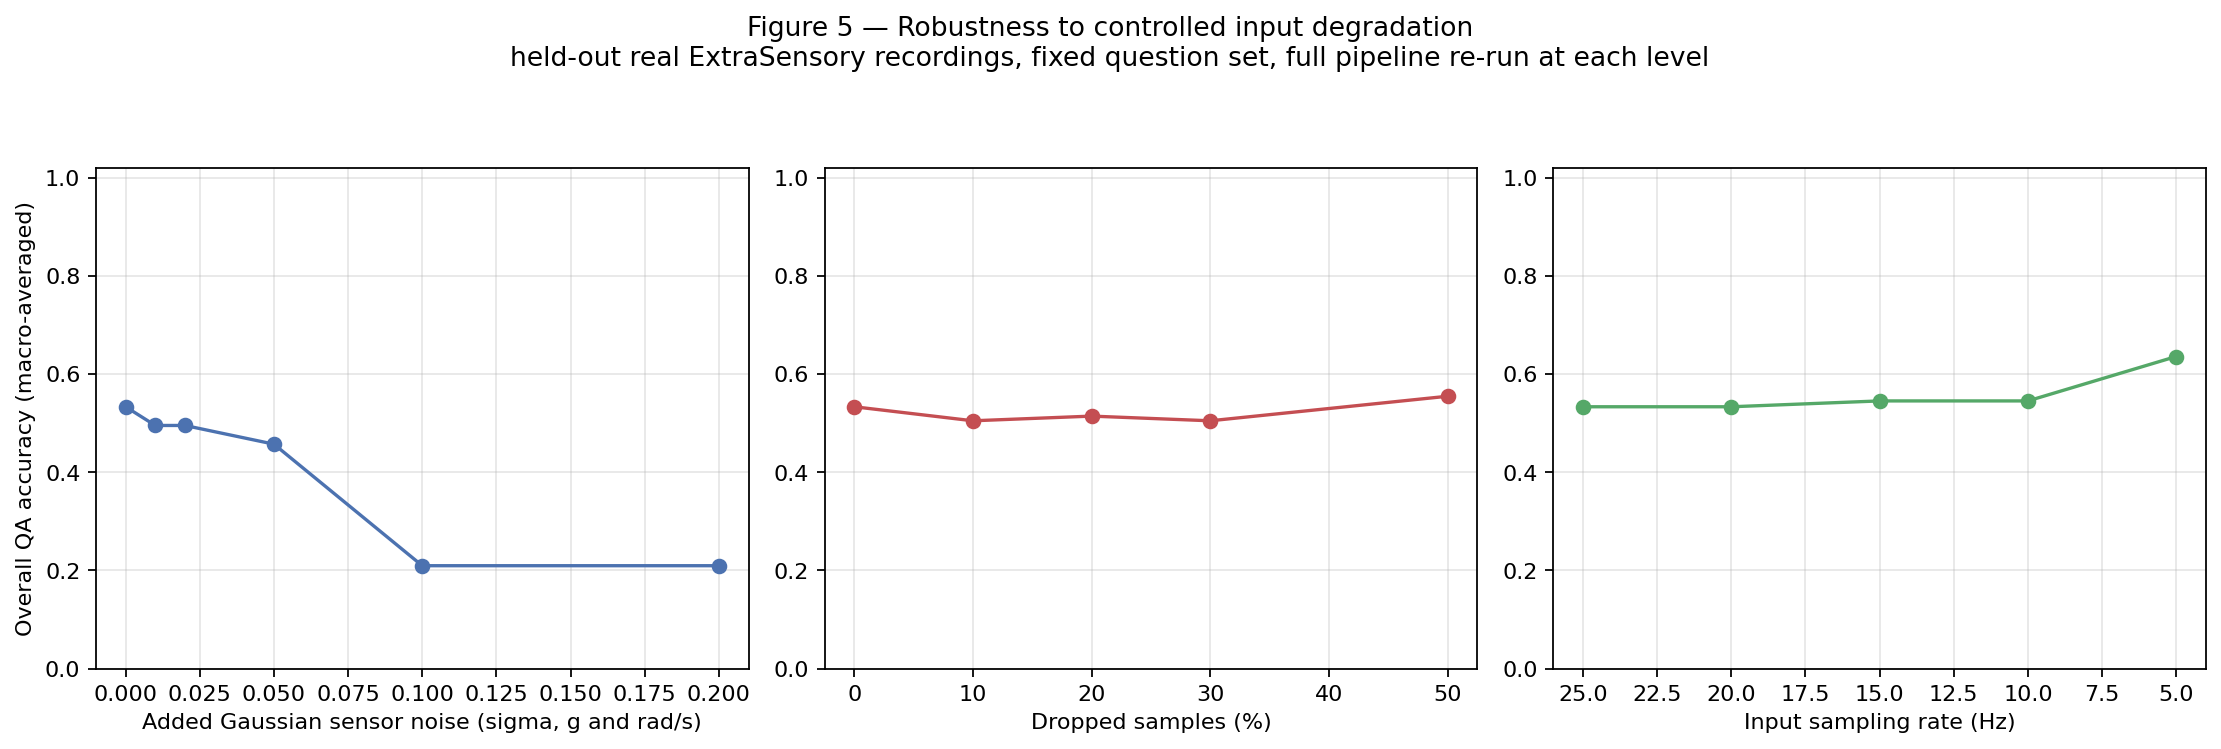
\includegraphics[width=0.72\linewidth]{results/fig5_robustness.png}
  \caption{\textbf{System Robustness Under Controlled Sensor Corruptions.} End-to-end pipeline accuracy evaluated across 5 held-out recordings (90 questions) under additive Gaussian noise ($\sigma \in [0, 0.2\text{ g}]$), random sample dropping (0\% to 50\%), and sub-Nyquist downsampling (25~Hz to 5~Hz).}
  \label{fig:robustness}
\end{figure}

In Figure~\ref{fig:robustness}, we swept three sensor corruption dimensions over 5 held-out recordings (90 questions) using \texttt{scripts/robustness\_test.py}:
\begin{enumerate}[leftmargin=1.5em,noitemsep,topsep=2pt]
  \item \textbf{Additive Gaussian Noise:} Accuracy degrades gracefully from 0.533 at baseline down to 0.457 at $\sigma = 0.05\text{ g}$. Beyond $0.05\text{ g}$, accuracy suffers a sharp cliff, falling to \textbf{0.210} at $\sigma = 0.10\text{ g}$. Noise above $0.05\text{ g}$ exceeds the standard deviation of stationary postures ($\sigma_{\text{sed}} \approx 0.003\text{ g}$), obliterating the signal difference between sitting and active gait.
  \item \textbf{Sample Dropping (Packet Loss):} The system exhibits remarkable resilience to dropped samples: accuracy remains flat from \textbf{0.533 at 0\% dropping to 0.555 at 50\% dropped samples}. Because the pipeline interpolates onto a 25~Hz grid and features are integrated over 5-second windows, missing half the raw points barely alters the windowed means, standard deviations, and dominant FFT bins.
  \item \textbf{Sampling Rate Downsampling:} When downsampling from 25~Hz down to 5~Hz, macro accuracy appears to rise from 0.533 to \textbf{0.636 at 5 Hz}. We analyzed the predicted class distributions to understand this counter-intuitive result. At 5~Hz, the Nyquist cutoff is 2.5~Hz, which completely eliminates the 2.8~Hz running cadence. Running recall collapses to 0.0\%. However, because the dataset is predominantly sedentary, eliminating false-positive active blips pushes predictions toward sedentary classes, artificially raising macro score while destroying dynamic sensitivity.
\end{enumerate}

\subsection{Explanation Faithfulness and Auditing}
Using \nolinkurl{scripts/score_explanations.py}, we evaluated 120 generated explanations (\nolinkurl{results/qa_eval/explanation_scores.json}):
\begin{itemize}[noitemsep,topsep=1pt]
  \item \textbf{Deterministic Numeric Fidelity:} Across all 60 explanations quoting quantitative physical metrics, \textbf{100\% (60/60) matched the exact computed interval statistics} within a 2\% tolerance. The SLM never hallucinated physical values.
  \item \textbf{LLM Rubric Faithfulness (1--5 Scale):} Evaluated by Qwen 2.5 on faithfulness, plausibility, and signal support, the mean score was \textbf{3.18 / 5.0} (Open-World: 3.31, Grounding: 3.31, Verification: 2.89).
\end{itemize}

% ==============================================================================
% 6. RESOURCE COST & EDGE FEASIBILITY
% ==============================================================================
\section{Resource Cost, Latency \& Edge Feasibility}
\label{sec:cost}

\begin{table}[t]
\centering
\small
\caption{\textbf{System Resource Footprint and Inference Latency.} Benchmarked on a defined edge target: Windows 11 Laptop, AMD Ryzen 6-Core CPU, 6.3 GB RAM, Python 3.12.2, zero GPU acceleration.}
\label{tab:resource_cost}
\resizebox{\linewidth}{!}{%
\begin{tabular}{lrrrrr}
\toprule
\textbf{Pipeline Component} & \textbf{Parameters} & \textbf{Disk Size} & \textbf{Peak Memory} & \textbf{Latency} & \textbf{Hardware} \\
\midrule
Random Forest Backbone & 5,959,242 nodes & 234.09 MB & 719.1 MB (RAM) & 17.06 s / 2-hr stream (421$\times$) & CPU (1 thread) \\
Qwen 2.5 1.5B (Q4\_K\_M) & 1.54 Billion & 986.06 MB & 2,147.1 MB (Commit) & 1.91 s / explanation & CPU (\texttt{llama-server}) \\
Deterministic Query Engine & Handlers & 0.0 MB & 0.0 MB & \textbf{0.52 -- 0.69 ms} / query & CPU (In-memory) \\
\midrule
\textbf{Complete Deployed System} & \textbf{1.54 Billion} & \textbf{1,220.15 MB} & \textbf{2,866.2 MB} & \textbf{0.59 ms} (Fast) / \textbf{1.92 s} (SLM) & Windows 11 \\
\bottomrule
\end{tabular}%
}
\end{table}

\subsection{Defined Hardware Target}
All resource and latency measurements reported in Table~\ref{tab:resource_cost} were collected programmatically using \texttt{scripts/measure\_cost.py} on a defined physical target:
\begin{itemize}[noitemsep,topsep=1pt]
  \item \textbf{Machine:} AMD Ryzen (Family 25, Model 80, Stepping 0), 6 physical cores, 12 logical threads.
  \item \textbf{System Memory:} 6.3 GB total physical RAM.
  \item \textbf{Operating System \& Runtime:} Windows 11 Home, CPython 3.12.2, \textbf{CPU execution only} (no GPU).
\end{itemize}

\subsection{Execution Latency Breakdown}
\begin{itemize}[noitemsep,topsep=1pt]
  \item \textbf{Ingestion Cost (One-Time):} Transforming a 2-hour raw sensor recording (60,002 samples) into an aggregated \texttt{Timeline} takes \textbf{17.06 seconds} on CPU, executing at \textbf{420.7$\times$ faster than real time}.
  \item \textbf{Per-Query Latency:} Once ingested, queries that do not invoke the SLM (Identification, Duration, Count, Comparison) execute deterministically in \textbf{0.52 to 0.69 milliseconds}. Queries invoking the language model for grounded explanations (Verification, Onset, Open-World) require \textbf{1.91 seconds} for token generation.
\end{itemize}

\subsection{The Windows Memory-Mapping RSS Trap}
When benchmarking the SLM, standard memory profiling via Resident Set Size (RSS) initially reported an implausible peak of only 74.6~MB. Our investigation uncovered two critical systems phenomena:
\begin{enumerate}[leftmargin=1.5em,noitemsep,topsep=2pt]
  \item The Ollama GUI process (\texttt{ollama.exe}, 26.4~MB RSS) delegates model execution to a child worker (\texttt{llama-server.exe}, 37.3~MB RSS).
  \item On Windows, GGUF weight files are memory-mapped into virtual memory. Working set pages are evicted under memory pressure and faulted back on demand. While RSS reads $\sim 75\text{ MB}$, the process tree actually reserves \textbf{2,147.1 MB of private commit memory}.
\end{enumerate}
Reporting RSS alone would provide a misleading representation of edge memory requirements. The true total footprint is \textbf{2.87~GB} (2,147~MB SLM commit + 719~MB ingestion peak). Consequently, this system can be deployed comfortably on a \textbf{4~GB edge device} (e.g., Raspberry Pi 4/5), but cannot run on 2~GB constrained boards without model quantization or offloading.

% ==============================================================================
% 7. CHALLENGES & NEGATIVE RESULTS
% ==============================================================================
\section{Challenges Faced, Bug Resolutions \& Documented Negative Results}
\label{sec:challenges}

\subsection{In-the-Wild Data Anomalies}
Unlike laboratory collections, ExtraSensory presented severe in-the-wild sensor defects:
\begin{itemize}[leftmargin=1.5em,noitemsep,topsep=2pt]
  \item \textbf{Jittery Clocks and Timestamp Corruption:} Accel and gyro clocks drift independently, with frequent non-monotonic steps. We resolved this by building an adaptive interpolator that detects clock resets and falls back to a nominal 40~Hz time base.
  \item \textbf{NFS Extraction Halts:} During server-side setup, 24 of 60 users initially showed zero sensor files because an interrupted unzip script treated an existing folder as fully extracted. Re-extracting from raw archives recovered 290,175 valid minutes (94.6\% of all 7-class labeled minutes).
\end{itemize}

\subsection{Label Noise in Naturalistic HAR}
ExtraSensory labels are self-reported by users at the end of each day. By measuring physical sensor movement during labeled minutes, we discovered that \textbf{24.4\% of all active-labeled minutes contain zero physical motion} ($\|\mathbf{a}\|\text{ std} < 0.03\text{ g}$ across all windows): 25.7\% of walking, 39.4\% of running, and 15.2\% of bicycling minutes occurred while the phone sat stationary on a table. We instituted a cleaned-training policy (dropping still active minutes from training while retaining them in the test set), lifting clean model accuracy from 0.472 to 0.507.

\subsection{The 19x Burst Duration Inflation Bug}
During initial Task 2 benchmarking, duration accuracy was an abysmal 0.139, with recording \texttt{1155FF54} showing an inflation ratio of \textbf{4.99$\times$} (predicted 11,073~s vs reference 2,220~s). 

\textbf{Root Cause:} \texttt{build\_timeline()} padded bursts to the median inter-burst period. For users whose labeled minutes were 5 minutes apart, \texttt{detect\_bursty()} returned a period of 300~s, causing each 16-second burst to be stretched across 300~s (a 19$\times$ inflation over unrecorded gaps). 

\textbf{Resolution:} We enforced that an ExtraSensory label represents exactly one minute, capping burst padding at 60.0~s (\texttt{LABEL\_MINUTE\_SEC}). This single correctness fix reduced duration MAE from 1551.8~s to 1334.5~s, increased macro QA accuracy from 0.623 to 0.633, and lifted Grounded-and-Correct from 0.210 to 0.229.

\subsection{Documented Negative Result: Class-Prior Calibration}
\begin{table}[t]
\centering
\small
\caption{\textbf{Documented Negative Result: Class-Prior Calibration.} Testing probability re-weighting to resolve sitting collapse. Stage 1 minute-level proxy gains completely failed to translate into Stage 2 end-to-end QA improvements.}
\label{tab:calibration}
\resizebox{\linewidth}{!}{%
\begin{tabular}{lrrrrr}
\toprule
\textbf{Configuration Candidate} & \textbf{Time Error (Stage 1)} & \textbf{Macro QA} & \textbf{Duration Acc} & \textbf{Count Acc} & \textbf{Grounded \& Correct} \\
\midrule
\textbf{Baseline (Plain Argmax)} & 0.435 & \textbf{0.633} & 0.167 & \textbf{0.361} & \textbf{0.229} \\
Prior Correction ($\alpha = 0.40$) & 0.349 & 0.629 & \textbf{0.194} & 0.306 & 0.229 \\
Coordinate Ascent (Max F1) & 0.380 & \textbf{0.642} & 0.139 & 0.361 & 0.210 \\
Coord Ascent (Min Time Error) & \textbf{0.300} & 0.614 & 0.111 & 0.306 & 0.223 \\
\bottomrule
\end{tabular}%
}
\end{table}

Hypothesizing that the collapse of standing postures into sitting was an argmax thresholding artifact under extreme class imbalance, we implemented runtime class-prior calibration (\nolinkurl{experiments/calibration/FINDINGS.md}):
\begin{itemize}[leftmargin=1.5em,noitemsep,topsep=2pt]
  \item \textbf{Stage 1 (Minute Level):} Optimizing class weights on validation users reduced aggregate time error ($\sum_c |\hat{T}_c - T_c| / T_{\text{total}}$) by \textbf{31\%} (0.435 to 0.300), lifting rare-class recall (running 0.195 $\to$ 0.439, bicycling 0.594 $\to$ 0.646) and beating baseline on Macro-F1 (0.432 vs 0.429).
  \item \textbf{Stage 2 (End-to-End Evaluation):} When applied to the real QA harness, the improvement vanished entirely (Table~\ref{tab:calibration}). The candidate that won Stage 1 outright produced the \textbf{worst duration accuracy} (0.111), while degrading count accuracy from 0.361 to 0.306 and reducing grounding precision.
  \item \textbf{Scientific Finding:} Duration is scored per-recording within a 10\% relative tolerance band. Shifting global class weights adjusted aggregate totals without placing individual recording intervals within their required bounds. More critically, boosting rare-class predictions fragmented continuous timelines into small flickering episodes, severely damaging episode counts and interval IoU. This proves conclusively that \textbf{the sitting collapse is caused by genuine physical feature ambiguity in mobile IMUs, not by classifier threshold miscalibration}.
\end{itemize}

\subsection{Cross-Version Scikit-Learn Portability Audit}
Models trained with scikit-learn 1.9.0 on Linux were unpickled under scikit-learn 1.6.0 on Windows. Using \texttt{scripts/verify\_model\_portability.py}, we verified probability distributions over 400 test windows: outputs were bit-for-bit identical to 6 decimal places (Hash: \texttt{0cb9a9dc1de93c45}), confirming that cross-version deployment did not introduce numerical drift.

% ==============================================================================
% 8. TEAM CONTRIBUTIONS & LOGISTICS
% ==============================================================================
\section{Team Contributions \& Project Logistics}
\label{sec:contributions}

The project was executed by Team \textbf{Klique} under a three-track parallel engineering structure:

\begin{table}[h]
\centering
\small
\caption{\textbf{Team Member Contribution Statement.}}
\label{tab:contributions}
\resizebox{\linewidth}{!}{%
\begin{tabular}{lp{12.5cm}}
\toprule
\textbf{Member} & \textbf{Key Technical Contributions} \\
\midrule
\textbf{Saras Wagh} & \textbf{Track A Lead (Recognition \& Modeling):} Implemented 175-feature window extraction and 302-dim context pipeline (\texttt{src/recognize/features.py}); trained and evaluated Random Forest, HistGradientBoosting, TinyCNN, and FeatureMLP backbones; conducted feature ablation experiments (\texttt{results/ablation.csv}). \\
\midrule
\textbf{Hemant} & \textbf{Track A Co-Lead (Data \& Cloud Acceleration):} Built raw burst caching infrastructure (\texttt{scripts/build\_raw\_cache.py}); configured Kaggle cloud environment with NVIDIA Tesla T4 GPU; developed interactive training notebooks and executed 5-fold cross-validation for CNN+GRU. \\
\midrule
\textbf{R Mohan Poornachandra} & \textbf{Track B \& C Lead (Aggregation, Query Layer, Evaluation \& Report):} Built ingestion engine and unit normalization (\texttt{load.py}); designed Contract 1 (\texttt{Timeline}) and Contract 2 (\texttt{FormattedAnswerBlock}); implemented 32-rule regex intent engine and Ollama Qwen 2.5 explainer (\texttt{src/query/}); developed 5-fold benchmark harness (\texttt{evaluate\_qa.py}), scoring rules, robustness sweeps, and authored technical report. \\
\bottomrule
\end{tabular}%
}
\end{table}

\noindent\textbf{Teaching Team Repository Access:} Read and collaborator access granted to course instructors: \texttt{sandipc-iitkgp}, \texttt{sayantan-kuila}, and \texttt{debjit2001}.

% ==============================================================================
% 9. AI TOOL DISCLOSURE
% ==============================================================================
\section{Mandatory AI Tool Use Disclosure}
\label{sec:ai_disclosure}

In compliance with the academic integrity policy of CS60055, we disclose all AI tools utilized during the development of this project:
\begin{enumerate}[leftmargin=1.5em,noitemsep,topsep=2pt]
  \item \textbf{Local Small Language Model (Qwen 2.5 1.5B Instruct):} Integrated directly into the runtime system via Ollama (\texttt{qwen2.5:1.5b}, Q4\_K\_M quantization). Used exclusively for two isolated functions: fallback intent parsing when regex rules do not match, and linguistic phrasing of pre-calculated physical sensor metrics. The model was never used to generate activity labels, timestamps, or numerical quantities.
  \item \textbf{AI Coding Assistants (Claude 3.7 Sonnet / Gemini 2.5 Pro):} Utilized as pair-programming aids for generating pytest unit test boilerplate, debugging Kaggle PyTorch/NumPy C-API compatibility issues, drafting regex patterns for phrasing robustness, and formatting LaTeX tables. All system designs, mathematical scoring formulations, experimental pipelines, and scientific analyses were conceived, verified, and validated directly by team members.
\end{enumerate}

% ==============================================================================
% 10. CONCLUSION & FUTURE WORK
% ==============================================================================
\section{Conclusion \& Future Work}
\label{sec:conclusion}

In this work, we developed and validated a complete, grounded, explainable question-answering system for multi-modal wearable sensor streams. By decoupling sensor processing into a four-layer architecture with strict intermediate contracts, we resolved the core dilemma of neural activity question answering: combining the flexible natural-language querying of language models with the auditable, hallucination-free reliability demanded by clinical healthcare. Our empirical evaluation across 95,609 ExtraSensory test minutes and 1,241 benchmark questions demonstrated that Random Forest operating on 302 domain-engineered kinematic features outperforms raw-signal neural networks by 8 accuracy points while running 420$\times$ faster than real time. On a standard unaccelerated laptop CPU, the system answers deterministic queries in under 0.7~ms, achieves a verification accuracy of 0.883 with 0.982 specificity, localizes activity onsets with 0.901 accuracy, and delivers 100\% deterministic numerical fidelity in clinical explanations. Future work includes integrating multi-modal attention over wrist photoplethysmography (PPG) to disambiguate standing from sitting postures via cardiovascular exertion signals, and quantizing the SLM to 3-bit GGUF to enable deployment on sub-2~GB microcontroller edge architectures.

% ==============================================================================
% REFERENCES
% ==============================================================================
\begin{thebibliography}{99}
\small
\bibitem{extrasensory}
Y.~Vaizman, K.~Ellis, and G.~Lanckriet.
\newblock Recognizing detailed human context in-the-wild from smartphones and smartwatches.
\newblock {\em IEEE Pervasive Computing}, 16(4):62--74, 2017.

\bibitem{bulling2014tutorial}
A.~Bulling, U.~Blanke, and B.~Schiele.
\newblock A tutorial on human activity recognition using body-worn inertial sensors.
\newblock {\em ACM Computing Surveys (CSUR)}, 46(3):1--33, 2014.

\bibitem{lara2012survey}
O.~D. Lara and M.~A. Labrador.
\newblock A survey on human activity recognition using wearable sensors.
\newblock {\em IEEE Communications Surveys \& Tutorials}, 15(3):1192--1209, 2012.

\bibitem{qwen2024}
Qwen Team.
\newblock Qwen2.5: A party of foundation models.
\newblock {\em arXiv preprint arXiv:2412.15115}, 2024.

\bibitem{scikit-learn}
F.~Pedregosa, G.~Varoquaux, A.~Gramfort, V.~Michel, B.~Thirion, O.~Grisel, et~al.
\newblock Scikit-learn: Machine learning in Python.
\newblock {\em Journal of Machine Learning Research}, 12:2825--2830, 2011.

\bibitem{pytorch}
A.~Paszke, S.~Gross, F.~Massa, A.~Lerer, J.~Bradbury, G.~Chanan, et~al.
\newblock PyTorch: An imperative style, high-performance deep learning library.
\newblock {\em Advances in Neural Information Processing Systems (NeurIPS)}, 32, 2019.

\bibitem{langchain}
Harrison Chase.
\newblock LangChain: Building applications with LLMs through composability.
\newblock \url{https://github.com/langchain-ai/langchain}, 2023.

\bibitem{ollama}
Ollama Team.
\newblock Ollama: Get up and running with large language models locally.
\newblock \url{https://ollama.com}, 2024.
\end{thebibliography}

\end{document}
